\documentclass{beamer}
\usepackage{HECbeamer}
% \usepackage{pgfpages}
% \pgfpagesuselayout{4 on 1}[letterpaper, landscape, border shrink=5mm]
\title[\color{white}{MATH 60604A \S~7c - Kaplan--Meier estimator}]{\texorpdfstring{MATH 60604A \\Statistical modelling \\ \S~7c - Kaplan$-$Meier estimator}{MATH 60604A \\ Statistical modelling \\ \S~7c - Kaplan-Meier estimator}}
\author{Léo Belzile}
\institute{HEC Montréal\\
Department of Decision Sciences}
\date{} 

\begin{document}
\frame{\titlepage}
% \begin{frame}
% \frametitle{Estimateur Kaplan--Meier}
% \begin{itemize}
% % \item Les méthodes d'analyse de survie sont spécifiquement conçues pour être en mesure de bien prendre en compte de la censure.
% \item L'un des estimateurs les plus couramment utilisés pour estimer la fonction de survie en présence de censure à droite non-informative est l'estimateur de \alert{Kaplan--Meier}.
% \item L'estimateur de Kaplan--Meier  est \alert{non-paramétrique}, c'est-à-dire, on ne fait pas d'hypothèse sur la loi de probabilité sous-jacente de la variable réponse $T_i$.
% \end{itemize}
% %    
% % \item \footnotesize{Notez qu'il existe de nombreuses méthodes pour estimer les courbes de survie. Par exemple, certains modèles paramétriques comprennent le modèle de Weibull, le modèle log-normal, etc. Nous ne verrons pas ces modèles.}
% 
% \end{frame}

\begin{frame}
\frametitle{Notation}
We consider a continuous random variable $T$ and an associated sample of size $n$.
\begin{itemize}
%\item Suppose we have $n$ subjects, for which we either observe the time until the event, or a (right) censored time.
\item Suppose that there are $D$ distinct event times
\item Let $0 \leq t_1 < t_2 < \cdots < t_D$ denote these ordered $D$ failure times. 
\item Let $r_j$ denote the number of individuals who are \emph{at risk} at time $t_j$. 
\bi
\item That is, these individuals have not had experienced the event (nor been censored) before time $t_j$. 
\item Thus, $r_j$ is the number of known survivors just before time $t_j$ who are ``at risk'' of experiencing the event at time $t_j$.
\ei
\item Let $d_j \in \{0, \ldots, r_j\}$ denote the number of failures at time $t_j$ (there are $d_j$ deaths at time $t_j$). 
\end{itemize}
\end{frame}
\begin{frame}
\frametitle{Derivation of Kaplan--Meier estimator}
 The probability of dying in the time window $(t_j, t_{j+1}]$ given survival until $t_j$ is 
 \begin{align*}
  h_j = \P{t_j < T \leq t_{j+1} \mid T > t_j} 
%   \\& = \frac{\P{t_j < T \leq t_{j+1}}}{\P{T > t_j} }
%   \\& 
  = \frac{S(t_j) - S(t_{j+1})}{S(t_j)}.
 \end{align*}
This recursion yields \begin{align*}
S(t) = \prod_{j: t_j < t} (1-h_j).
\end{align*}
The Kaplan--Meier estimator is is \alert{non-parametric}: 
\bi \item it does not assume any underlying probability distribution for the variable $T_i$
\item rather, the conditional probabilities $\{h_j\}_{j=1}^D$ are treated as parameters of the model.
\ei
\end{frame}

\begin{frame}
\frametitle{Likelihood for the discrete observations}
\bi \item Each failure at time $t_j$ contributes $h_j$ to the likelihood
\bi \item the probability of failure at $t_j$ given survival in the previous time interval. \ei 
\item 
The likelihood contribution of survivors at time $t_j$ is $1-h_j$.
\item 
We may write the log likelihood as
\begin{align*}
 \ell(\bs{h}) = \sum_{j=1}^D \{ d_j \ln(h_j) + (r_j-d_j)\ln(1-h_j)\},
\end{align*}
the sum of contributions of binomial variables at time $t_j$.
\ei
\end{frame}
\begin{frame}
\frametitle{Optimizing the survival probabilities}
\begin{itemize}
\item Differentiating $\ell(\bs{h})$ with respect to  $h_j$, we find $\widehat{h}_j = d_j/r_j$.
\item The Kaplan--Meier estimator of the survival function is
\begin{align*}
\widehat{S}(t) = \prod_{t_j < t} \left( 1 - \frac{d_j}{r_j} \right)                                                                      \end{align*}
\item 
Intuition: $d_j/r_j$ is the sample proportion of death at time $t_j$ relative to the total population still alive at time $t_j$.
\end{itemize}
\end{frame}

\begin{frame}
\frametitle{Example}
The \code{breastcancer} data from Sedmak \textsl{et al.} (1989) contain informations on patients with breast cancer, including the following variables:
\begin{itemize}
 
\item \code{time}: time until death, or end of study  (in months)
\item \code{death}: indicator variable for death either \code{0} for right-censored times or \code{1} for death
\item \code{im}: response to immunohistochemical examination, either negative (\code{0}) or positive (\code{1})
\end{itemize}
%    
% 
% \item[] \tiny{
% Ces données proviennent de (), comme l'illustre le livre \emph{Survival Analysis: Techniques for Censored and Truncated Data} par John P. Klein \& Melvin L. Moeschberger}
% \end{itemize}
\end{frame}


\begin{frame}
\frametitle{Descriptive statistics for \code{breastcancer}}
\begin{center}
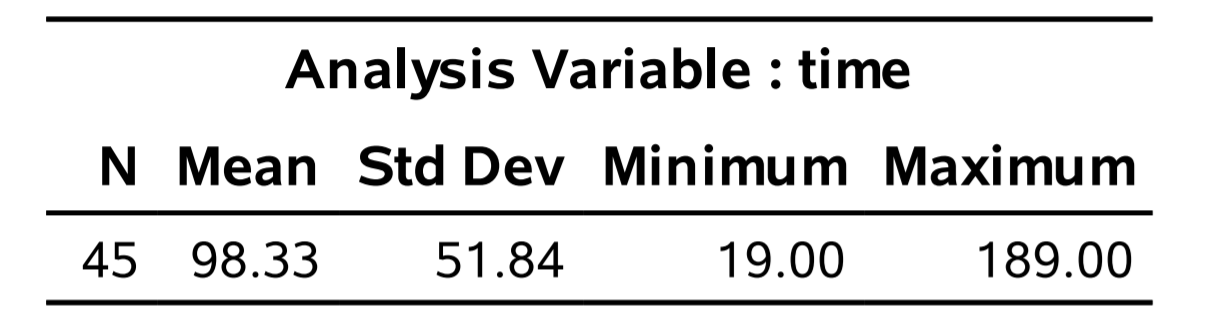
\includegraphics[width = 0.6\textwidth]{img/c7/slides7e01}
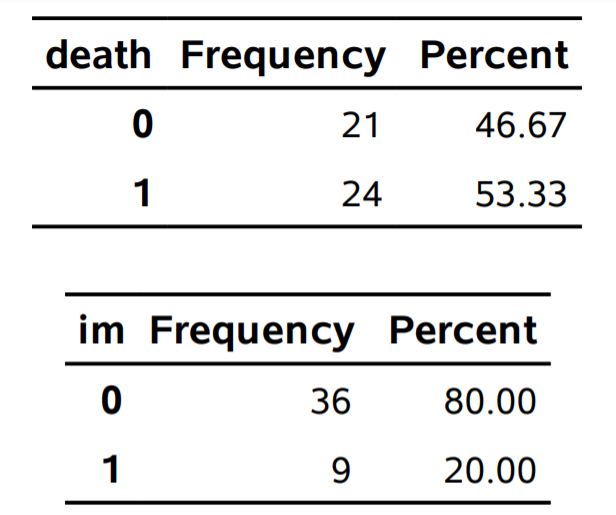
\includegraphics[width = 0.4\textwidth]{img/c7/slides7e02}
\end{center}
{
\footnotesize In practice, Kaplan--Meier estimator requires significant number observations to be a reliable approximation of the true survivor curve ($n \gg 1000$).

Keep in mind censored observations contribute less information than observed failure times.

}
\end{frame}


\begin{frame}[fragile]
\frametitle{Estimation of the survival function }

\begin{tcolorbox}[colback=white,colframe=hecblue,title= \SASlang{} code to fit the Kaplan--Meier estimator]
{\footnotesize 
\begin{verbatim}
proc lifetest data=statmod.breastcancer method=km plots=(s(cl));
time time*death(0);
run;
\end{verbatim}
}
\end{tcolorbox}
{ \footnotesize 
The \code{time} argument indicates both the response $T_i$ (\code{time}) and the right-censoring indicator $\delta_i$, with the reference in parenthesis for the right-censored observations (\code{death=0})

}
\end{frame}

\begin{frame}
\frametitle{Estimated survival function}
\begin{center}
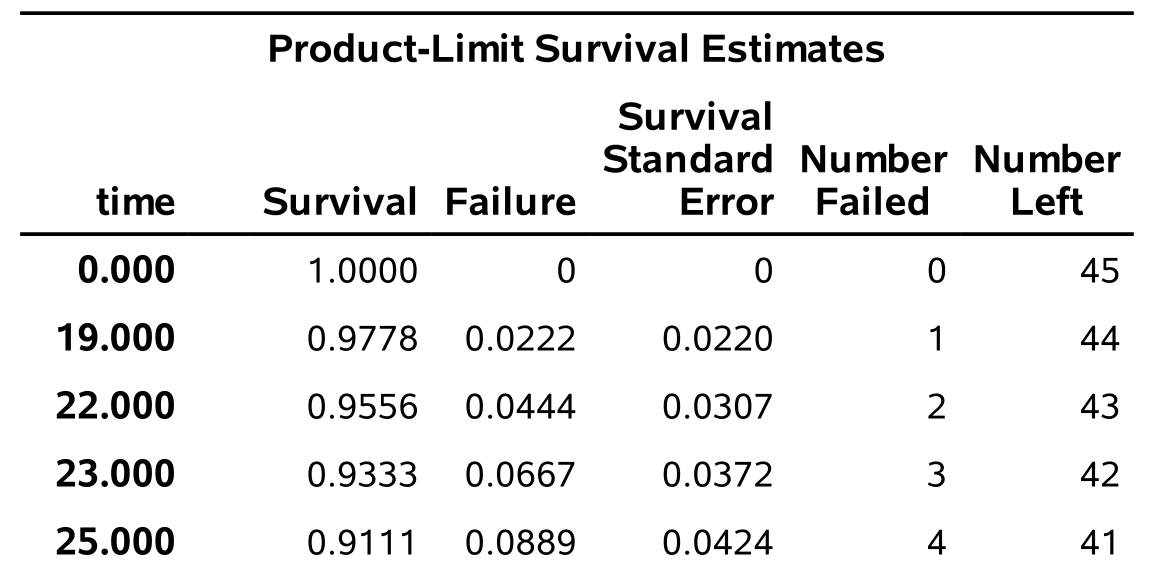
\includegraphics[width = 0.6\textwidth]{img/c7/slides7e03}
\begin{align*}
 \vdots
\end{align*}
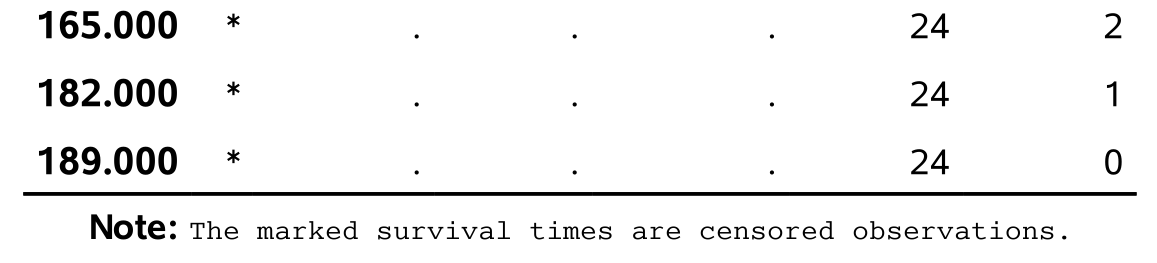
\includegraphics[width = 0.6\textwidth]{img/c7/slides7e04}
\end{center}
\end{frame}

\begin{frame}
\frametitle{Plot of the survival function}
\begin{center}
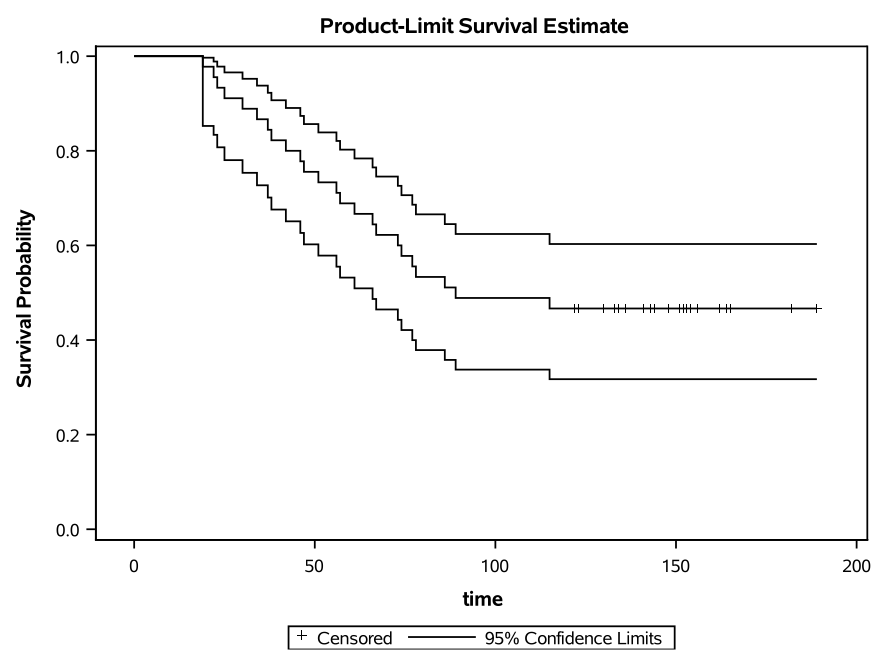
\includegraphics[width = 0.8\textwidth]{img/c7/slides7e05}
\end{center}
{ \footnotesize 

The survival curve is not consistent: $\widehat{S}(t)$ doesn't decrease to zero because the largest observed time is right-censored.


}
\end{frame}
% \begin{frame}
% \bi \bi
% \item On voit que la dernière observation de temps à $t=189$ est représenté par une coche dans le graphique car l'observation est censurée. 
% \item La dernière baisse de $\widehat{S}(t)$ sera à $t_D$: le plus grand temps de décès observé.  
% 
% \begin{center}
% \includegraphics[scale=0.6]{img/c7/btrial_plateau.png}
% \end{center}
% 
% \end{itemize}
% \end{itemize}
% \end{frame}

\begin{frame}
\frametitle{Breastfeeding duration}
The \code{breastfeeding} data from the National Longitudinal Survey of Youthcontains information on the time until which mothers stop breastfeeding from birth. We focus on the following explanatories:
\begin{itemize}
\item \code{duration}: duration of breast feeding (in weeks)
\item \code{delta}: indicator for completed breastfeeding 
\bi \item yes (\code{1}) 
\item right-censored (\code{0})
\ei
%\item \code{race}: race of mother (1=white, 2=black, 3=other)
%\item \code{poverty}: poverty status of mother (1=yes, 0=no)
%\item \code{smoke}: smoking status of mother at birth of child (1=yes, 0=no)
%\item \code{alcohol}: alcohol-drinking status of mother at birth of child (1=yes, 0=no)
%\item \code{agemth} age of mother at birth of child
%\item \code{ybirth} year of child's birth
%\item \code{yschool}: education level of mother (years of school)
%\item \code{pc3mth}: lack of prenatal care status (1= mother did not seek within first 3 months, 0=mother sought prenatal care in first three months of pregnancy)

\end{itemize}
\begin{center}
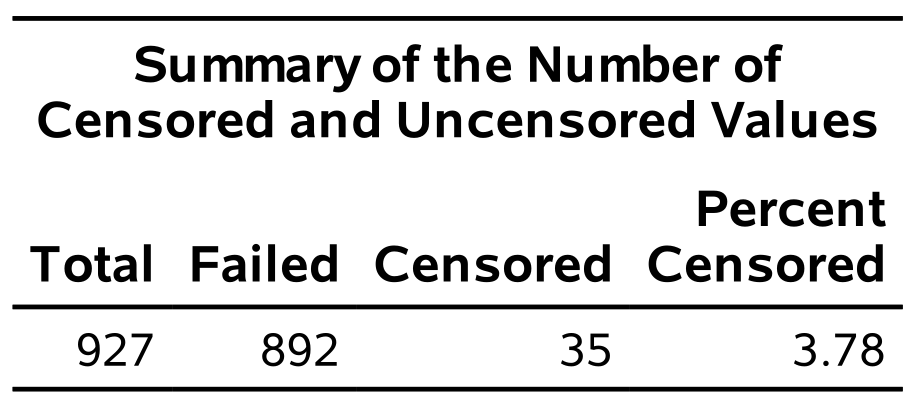
\includegraphics[width = 0.5\textwidth]{img/c7/slides7e09}
\end{center}
% 
% \item[] \tiny{Ces données proviennent de l'Enquête longitudinale nationale sur les jeunes, tels qu'illustrés dans le livre \emph{Survival Analysis: Techniques for Censored and Truncated Data} par John P. Klein \& Melvin L. Moeschberger}
% \end{itemize}
\end{frame}

\begin{frame}
\frametitle{Survival curve for \code{breastfeeding} data }

\begin{center}
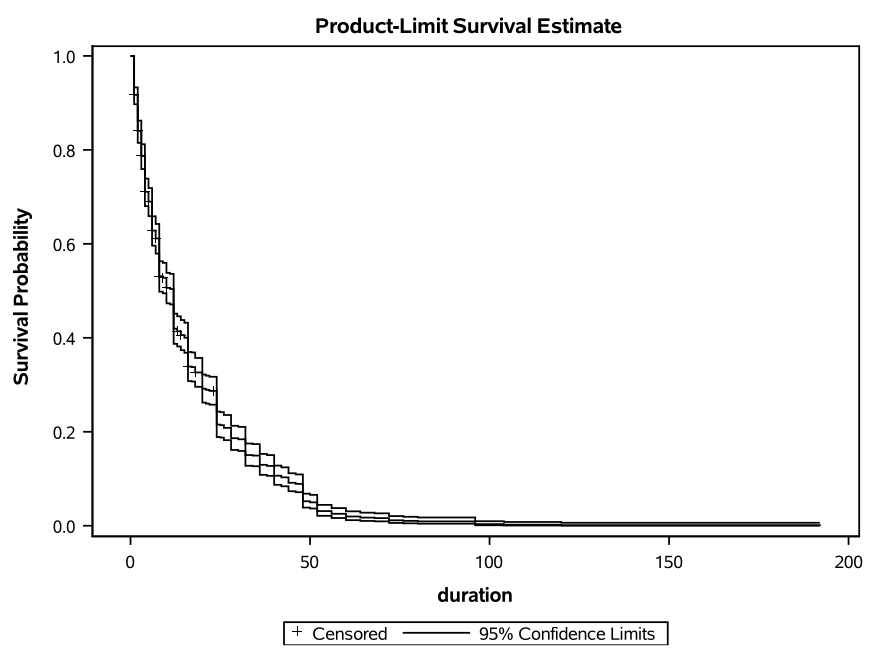
\includegraphics[width = 0.8\textwidth]{img/c7/slides7e08}
\end{center}
{\footnotesize $\widehat{S}(t)$ reaches zero because the largest survival time is observed, not censored.

}
\end{frame}
% 
% \begin{frame}
% \frametitle{Exemple}
% \begin{itemize}
% \item Dans cet exemple, la courbe de survie estimée atteint $0$. 
% \item C'est parce que le temps de survie le plus grand dans les données n'est pas censuré:
% 
%     
% 
% %\begin{center}
% \begin{tabular}{c c}
% %\begin{footnotesize}
% \code{duration} & \code{delta} \\
% 192 &  1
% %\end{footnotesize}
% \end{tabular}
% %\end{center}
% 
% \item La dernière baisse dans $\widehat{S}(t)$ atteindra zéro puisque le plus grand temps de survie observé dans les données est en fait le dernier temps d'événement $t_D$.  
% 
% \begin{center}
% \includegraphics[scale=0.6]{img/c7/bfeed_plateau.png}
% \end{center}
% 
% \end{itemize}
% \end{frame}

\begin{frame}[fragile]
\frametitle{Median survival time}
The median survival time is the time $t_M$ such that $S(t_m) = 0.5$.
\begin{itemize}
 \item That is, the median time $t_M$ is such that $50\%$ of people have survived until time $t_M$. 
\end{itemize}
 We can easily find this estimated median time by seeing where the horizontal line $\widehat{S}(t) = 0.5$ intersects the survival curve.
\begin{center}
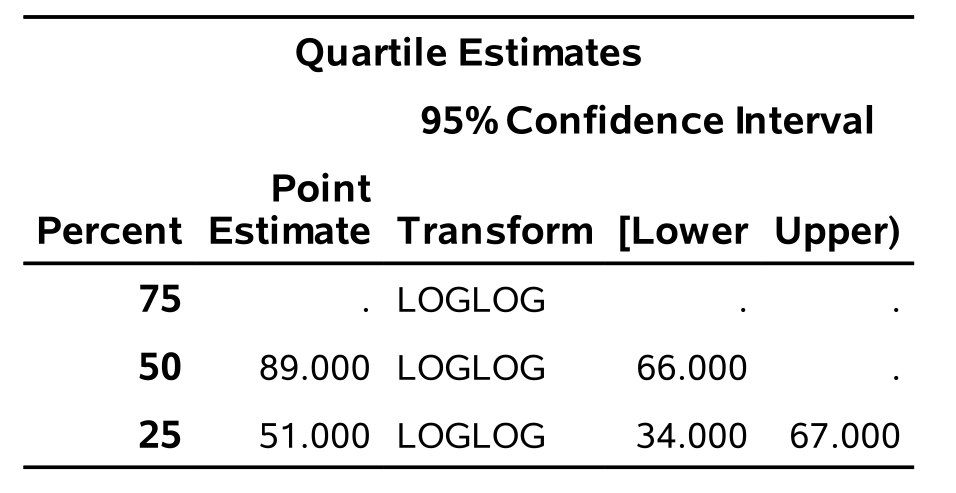
\includegraphics[width = 0.7\textwidth]{img/c7/slides7e07}
\end{center}

\end{frame}

% \begin{frame}[fragile]
% \frametitle{La médiane de survie}
% \begin{itemize}
% \item SAS va automatiquement calculer la médiane du temps de survie. 
% \item Dans les données sur les patients avec le cancer du sein, on obtient un temps de survie médian de $89$
%   
% \begin{center}
% \includegraphics[scale=0.4]{img/c7/btrial_km_median.png}
% \end{center}
% \item Notez que si le temps observé le plus long est \alert{censuré} et que la courbe de survie estimée atteint un plateau qui est plus \alert{élevé} que la ligne horizontale de $0.5$, alors nous ne pourrons pas estimer la médiane du temps de survie. 
% \begin{center}
% \includegraphics[scale=0.35]{img/c7/km_ex_no_med.png}
% \end{center}
% \end{itemize}
% \end{frame}


\begin{frame}
\frametitle{Mean survival time}
For a continuous positive random variable, $T>0$, it can be shown that 
\begin{align*}
\E{T} = \int_0^{\infty} S(t) \d t
\end{align*}
We can estimate the expected survival time $\E{T}$ simply by calculating the area under the survivor curve $\widehat{S}(t)$. 
\begin{itemize}
\item For example, the mean survival time for the breastfeeding data is $16.89$ weeks with standard error $0.614$ weeks.
\item If the largest recorded survival time is \alert{censored}, the estimated survival curve $\widehat{S}(t)$ will plateau and never reaches  $0$. The area under the curve is infinite!
\item  In this case, we can estimate instead the restricted mean survival time: $\E{\min\{T,\tau\}}$ for a chosen $\tau$. It amounts to calculating the average as if the curve dropped to $0$ at time $\tau$ (\code{rmst} option in \SASlang{}).
\end{itemize} 
\end{frame}
% 
% \begin{frame}
% \frametitle{Exemple}
% %\textbf{SAS output}
% \begin{itemize}
% \item Par défaut, \SASlang{} va estimer la moyenne du temps de survie o\`u l'estimation est limitée au plus grand temps d'événement observé $t_D$.
% \item Ex: pour les données sur les patients avec le cancer du sein, on obtient
%   
% \begin{center}
% \includegraphics[scale=0.5]{img/c7/btrial_km_mean.png}
% \end{center}
% \item Remarquez que SAS indique que la moyenne du temps de survie est \alert{sous-estimée} puisque l'estimation est limitée au plus grand temps d'événement, mais dans les données la plus grande observation est censurée\ldots
% \end{itemize}
% \end{frame}
% % 
% \begin{frame}[fragile]
% \frametitle{Exemple}
% \begin{itemize}
% \item Si on inclut l'option \code{rmst} en SAS, la moyenne limitée sera calculée, et l'estimation sera limitée à la plus grande valeur observée $t_{max}$, ou à un $\tau$ spécifié. 
% \end{itemize}
% \begin{tcolorbox}[colback=white,colframe=blue!75!black,title=Code SAS ]
% \begin{verbatim}
% proc lifetest data=modstat.btrial method=km
% plots=(s(cl)) rmst;
% time time*death(0);
% run;
% \end{verbatim}
% \end{tcolorbox}
% \begin{center}
% \includegraphics[scale=0.5]{img/c7/btrial_rmst.png}
% \end{center}
% \begin{itemize} 
% \item On voit que SAS sélectionne $\tau=189$, qui est le plus grand temps dans l'ensemble de données (observation censurée).
% \end{itemize}
% \end{frame}

\end{document}
